\documentclass[12pt,a4paper]{article}

% load packages
\usepackage{xcolor}
\usepackage{graphicx}
\usepackage{amsmath}
\usepackage{amsfonts}
\usepackage{amssymb}
\usepackage{parskip}
\usepackage{tikz}
\usepackage{listings}
\usepackage{hyperref}
\usepackage{algorithm}
\usepackage{algpseudocode}
\usepackage[left=2cm,right=2cm,top=2cm,bottom=2cm]{geometry}

% set code style
\definecolor{codegreen}{rgb}{0,0.6,0}
\definecolor{codegray}{rgb}{0.5,0.5,0.5}
\definecolor{codepurple}{rgb}{0.58,0,0.82}
\definecolor{backcolour}{rgb}{0.95,0.95,0.92}

% set lst style
\lstdefinestyle{mystyle}{
    backgroundcolor=\color{backcolour},   % 设置背景颜色
    commentstyle=\color{codegreen},
    keywordstyle=\color{magenta},
    numberstyle=\tiny\color{codegray},
    stringstyle=\color{codepurple},
    basicstyle=\ttfamily\footnotesize,    % 使用等宽字体
    breakatwhitespace=false,         
    breaklines=true,                 
    captionpos=b,                    
    keepspaces=true,                 
    numbers=left,                    
    numbersep=5pt,                  
    showspaces=false,                
    showstringspaces=false,
    showtabs=false,                  
    tabsize=2
}
\lstset{style=mystyle}


\title{Project 2 Report for Probelm 2.1}
\author{Zhu Liang}
\date{\today}

\begin{document}

\maketitle

\section{Project Description}
In this project, we undertake two primary tasks. 
The first task is to provide a detailed description of the algorithms behind five collective communication operations provided by MPI.
The description are provided in Section \ref{sec:mpi_buildin}.
The second task is an empirical comparison between the built-in \texttt{MPI\_Bcast} and a custom broadcast implementation named \texttt{MY\_Bcast()}.


\section{Algorithm Description}
\subsection{MPI Build-in Operations}
\label{sec:mpi_buildin}


\textbf{\texttt{MPI\_Bcast()}}: This function broadcasts a message from the process with the designated root rank to all other processes in the communicator. All processes must call this function, with matching arguments.

\textbf{\texttt{MPI\_Scatter()}}: This function distributes distinct blocks of data from the root process to each process in the communicator. The root sends data to itself as well as to the other processes.

\textbf{\texttt{MPI\_Allgather()}}: Each process sends its own data to all other processes and gathers data from all processes. At the end, every process has the data from all the other processes.

\textbf{\texttt{MPI\_Alltoall()}}: This function allows each process to send distinct data to every other process. It generalizes the functionality of both scatter and gather, with different data being sent to each process.

\textbf{\texttt{MPI\_Reduce()}}: All processes in the communicator contribute their own data, which is combined (reduced) into a single result using a specified operation, like sum, max, etc. The result is stored on the root process.


\subsection{Custom Broadcast Function: \texttt{MY\_Bcast()}}
In large-scale parallel computations, efficient data transfer across processes is paramount. 
A simple broadcast approaches, 
which involve a root process sending messages to every other process sequentially, 
can be inefficient, 
especially when the number of processes grows, 
leading to a linear time complexity of $O(n)$.

To enhance this, 
we leverage it with a binary tree structure. 
Here, each process communicates only with its parent and potential left and right children (when children exist). 
Thus, it works even when the number of processes is a full binary tree.
The root initiates the broadcast, and the message cascades down the tree, reaching all processes.
Pleasee refer to Figure \ref{fig:binary_tree} for an illustration of the binary tree structure when $P = 4$,
which is not a full binary tree.
This approach reduces the time complexity from $O(n)$ to $O(log(n))$.

For more details on the project structure and the implementation, 
please refer to the \texttt{README.md} file in the \texttt{project2} folder.

The pseudocode is shown below.
\begin{algorithm}
    \caption{Custom Broadcast Function Using Binary Tree}
    \begin{algorithmic}[1]
    \Procedure{MY\_ Bcast}{}
    \State \textbf{Get} rank and size of processes
        \If{current process rank is not \textit{root}}
            \State \textbf{Receive} content of buffer from \textit{parent} 
        \EndIf
        \If{\textit{left child} exists}
            \State \textbf{Send} content of buffer to \textit{left child} 
        \EndIf
        \If{\textit{right child}  exists}
            \State \textbf{Send} content of buffer to \textit{right child} 
        \EndIf
        \State \Return MPI\_SUCCESS
    \EndProcedure
    \end{algorithmic}
\end{algorithm}

\begin{figure}
    \centering
    \begin{tikzpicture}[
        every node/.style = {circle, draw},
        missing/.style={fill=gray!50, label=center:{\textbf{X}}, edge from parent/.style={draw=none}},
        phantom/.style={draw=none, edge from parent/.style={draw=none}},
        level distance = 15mm,
        level 1/.style = {sibling distance=40mm},
        level 2/.style = {sibling distance=20mm},
        level 3/.style = {sibling distance=10mm},
      ]
      
      \node {0}
        child[->] {node {1}
          child[->] {node {3}
            child[missing] {}
            child[missing] {}
          }
          child[phantom] {}
        }
        child[->] {node {2}
          child[missing] {}
          child[missing] {}};
      
    \end{tikzpicture}
    \caption{Binary Tree Structure when $P = 4$}
    \label{fig:binary_tree}
\end{figure}
  
  
  
\section{Results}
In the following tables, 
 we present the execution times for two different broadcast implementations: 
 \texttt{MPI\_Bcast} and \texttt{MY\_Bcast}. 
Please note that individual run times might vary depending on the specific runtime environment, 
but the general pattern observed should remain similar across different runs. 

Referring to Tables \ref{tab:mpi_bcast} and \ref{tab:my_bcast}, 
 we can see the aforementioned times for various $P$ and $N$ values.
Here, $P$ represents processor count and $N$ dictates size of data being 
broadcasted.

As part of our exercise to ensure accuracy in measurement, 
 we implemented a rigorous tactic to eliminate various factors that could 
 contribute to measurement errors. 
Specifically, for each pair of $N$ and $P$, 
 we performed 50,000 broadcast operations using the Bcast function,
 recorded the whole execution time, and then computed the average time. 
This repeated procedure allowed us to smooth out any potential anomalies - 
 such as inconsistent system performance or unexpected delays - 
 thereby providing us with a more reliable measure of typical execution time. 
We also add a warm-up phase before the actual measurement to ensure that 
 the system is fully warmed up and ready to deliver consistent performance.

Upon assessing the results, an intriguing pattern has surfaced. 
When $P=4$, \texttt{MY\_Bcast} exhibits shorter execution time compared to \texttt{MPI\_Bcast}. 
However, as $P$ increases beyond the value of 4, 
\texttt{MPI\_Bcast} begins to outperform \texttt{MY\_Bcast}, 
offering better performance. 
This suggests that \texttt{MPI\_Bcast } is potentially more beneficial for larger processor 
 counts, where it delivers improved broadcast times.

\begin{table}[!htb]
   \centering   
   \begin{tabular}{|c|c|c|c|c|}    
   \hline    
   & P = 4 & P = 7 & P = 28 & P = 37 \\   
   \hline    
   $N = 2^{10}$ & 0.000008s & 0.000011s & 0.000022s & 0.000026s \\   
   \hline    
   $N = 2^{12}$ & 0.000011s & 0.000020s & 0.000035s & 0.000045s \\  
   \hline    
   $N = 2^{14}$ & 0.000031s & 0.000048s & 0.000100s & 0.000143s \\   
   \hline    
   $N = 2^{16}$ & 0.000099s & 0.000156s & 0.000349s & 0.000564s \\   
   \hline    
   \end{tabular}    
   \caption{Average Execution time using \texttt{MPI\_Bcast}}    
   \label{tab:mpi_bcast}
\end{table}

\begin{table}[!htb]
   \centering    
   \begin{tabular}{|c|c|c|c|c|}    
   \hline    
   & P = 4 & P = 7 & P = 28 & P = 37 \\   
   \hline    
   $N = 2^{10}$ & 0.000007s & 0.000015s & 0.000031s & 0.000035s \\   
   \hline    
   $N = 2^{12}$ & 0.000010s & 0.000026s & 0.000053s & 0.000063s \\   
   \hline    
   $N = 2^{14}$ & 0.000022s & 0.000064s & 0.000152s & 0.000178s \\   
   \hline    
   $N = 2^{16}$ & 0.000065s & 0.000212s & 0.000477s & 0.000616s \\   
   \hline    
   \end{tabular}    
   \caption{Average Execution time using \texttt{MY\_Bcast}}    
   \label{tab:my_bcast}
\end{table}

\begin{figure}
    \centering
    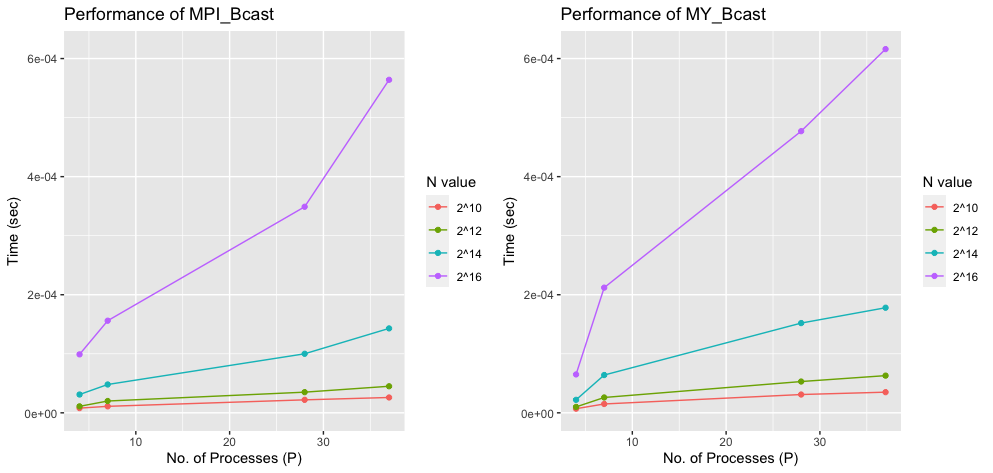
\includegraphics[width=0.9\textwidth]{Rplot01.png}
    \caption{Comparison of Execution Time between \texttt{MPI\_Bcast} and \texttt{MY\_Bcast}}
\end{figure}


\section{Analysis}

Based on the empirical results obtained,
 both \texttt{MPI\_Bcast()} and our custom implementation
 \texttt{MY\_Bcast()} demonstrate closely matched performance. 
This is a significant observation given that the \texttt{MY\_Bcast()} function 
 was optimized to operate in \(O(\log(n))\) time complexity, 
 using a binary tree approach.

Delving deeper into the specifics of the performance under different scenarios 
 reveals some noteworthy patterns.
When the processor count is very samll, the \texttt{MY\_Bcast()} function manages
 to edge out the native \texttt{MPI\_Bcast()} in terms of execution time. 
This could be attributed to the simplistic structure of the \texttt{MY\_Bcast()} function. 
Its binary tree-based broadcasting strategy doesn't involve complex computations 
 or arrangements for data broadcast, 
 which could potentially give it an advantage when dealing with a 
 smaller number of processors. 
The reduced communication overhead and streamlined data management in 
 these smaller settings might favor the less complicated design 
 of \texttt{MY\_Bcast()}, thereby leading to better performance 
 as compared to \texttt{MPI\_Bcast()}.

However, as we scale up and increase the processor count beyond 4, 
 the nature of these performance dynamics takes a noticeable shift. 
Under these circumstances, the native \texttt{MPI\_Bcast()} function starts 
 exhibiting superior performance over the \texttt{MY\_Bcast()}. 
It handles the increased parallelism better and delivers faster broadcast times. 

This phenomenon might be because MPI's built-in broadcast operation is 
 highly optimized for larger processor counts, 
 and it may employ sophisticated algorithms under the hood to 
 manage inter-processor communication efficiently. 
In contrast, 
 the simplistic binary-tree approach used in \texttt{MY\_Bcast()} might
 not scale equally well with an increasing number of processors.

\section*{File Notes}
The source code of the program is in the \texttt{project2} folder. 
For more details, please refer to the \texttt{README.md} file in the folder.

\end{document}
